\subsubsection{Stern-Gerlach Experiment}

\begin{mystadmonition}{mystAmber}{Slogan:}Stern-Gerlachundefineddemonstratedundefinedthatundefinedtheundefinedspinundefinedangularundefinedmomentumundefinedofundefinedelectronundefinedisundefinedquantized,undefinedwithundefinednumericalundefinedvaluesundefined$\pm \hbar /2$

\end{mystadmonition}

Considerundefinedtheundefinedfollowingundefinedexperimentalundefinedsetundefinedup:

\begin{figure}[!htbp]
\centering
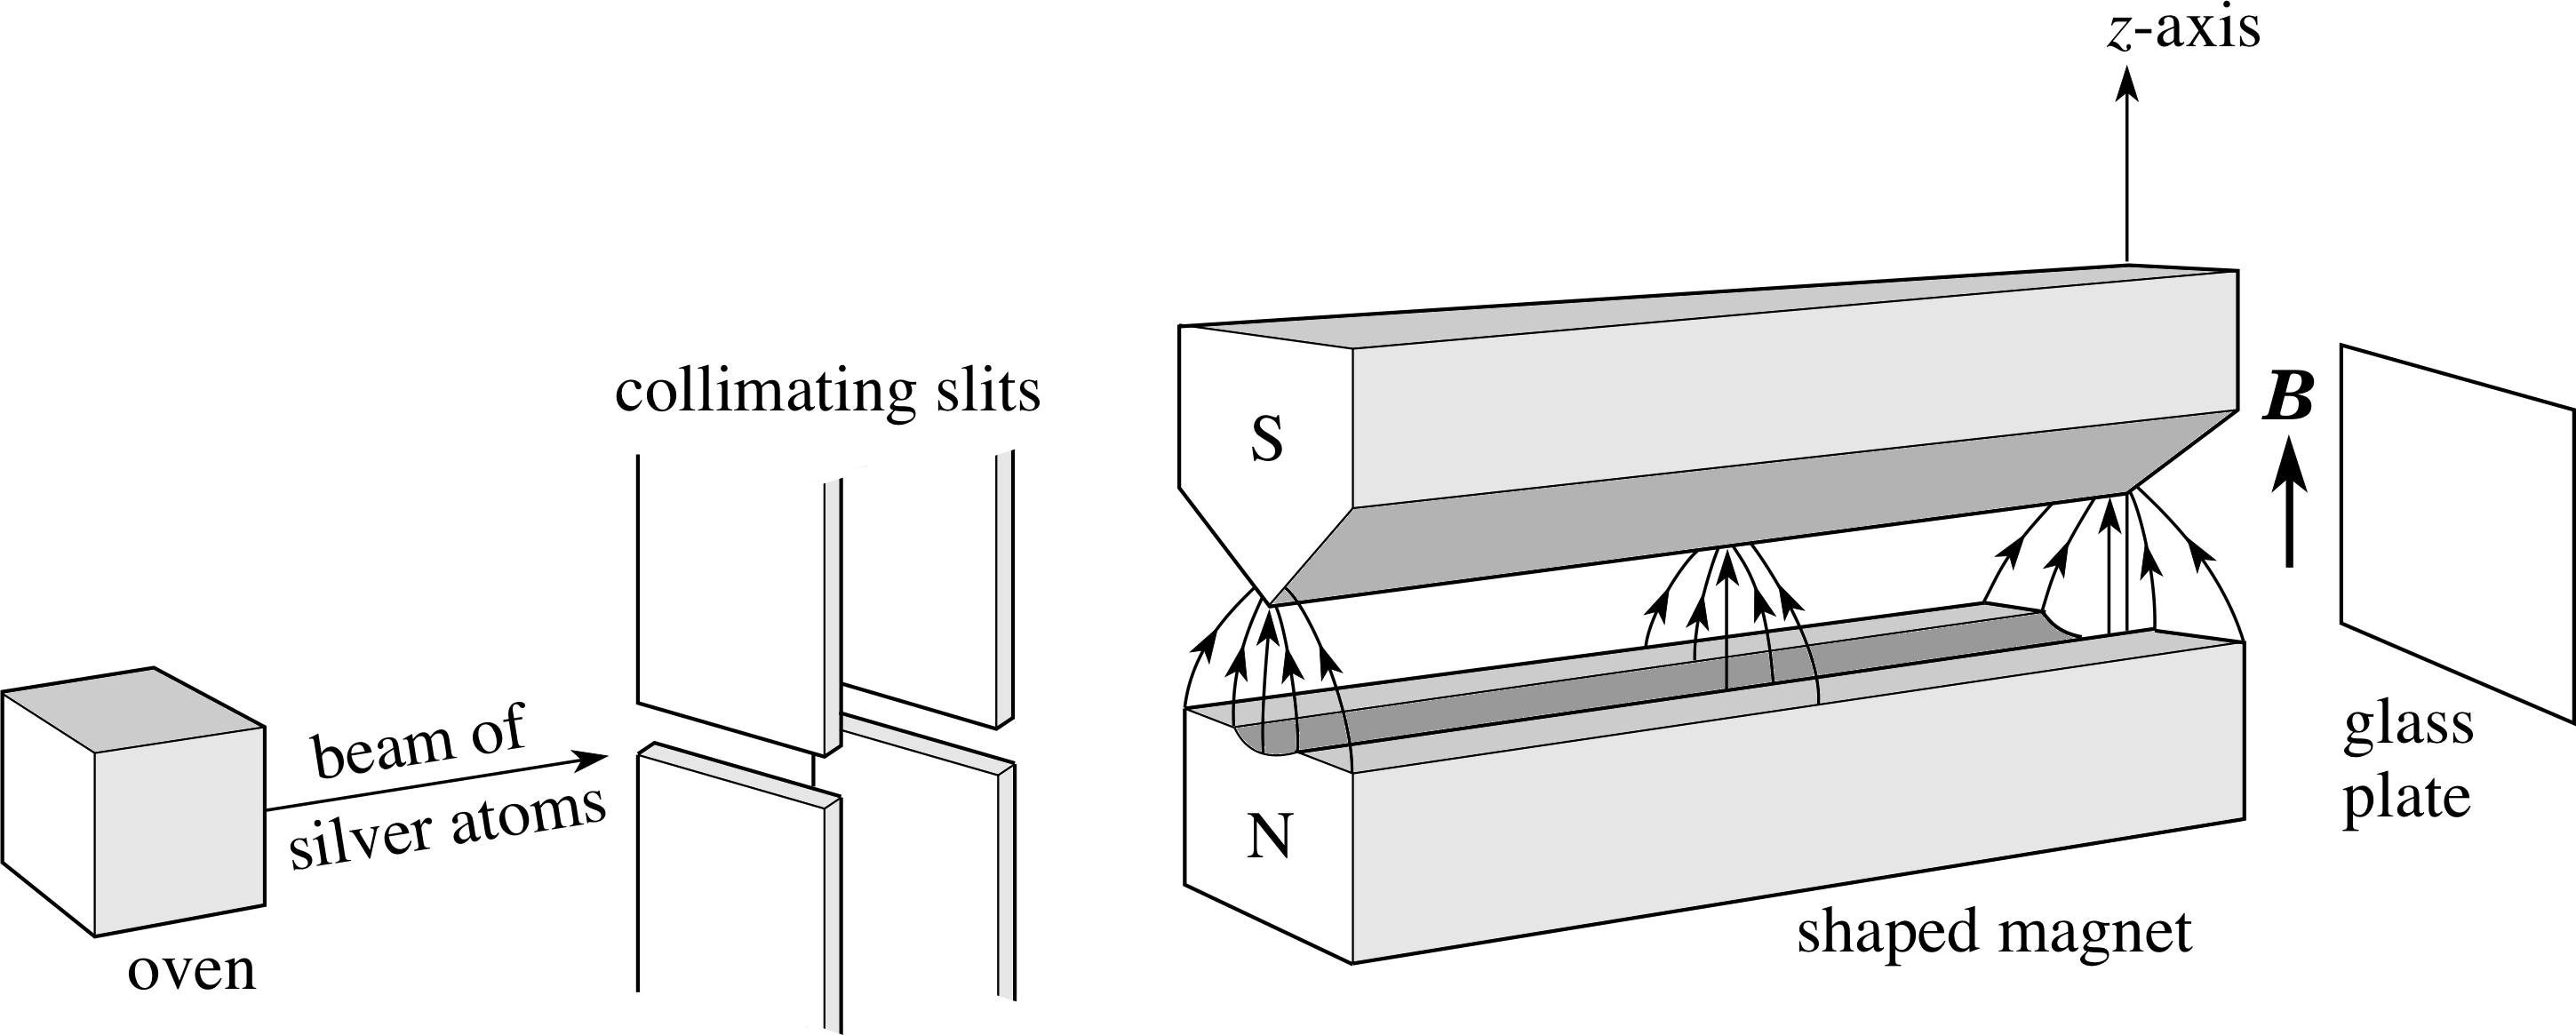
\includegraphics[width=0.7\linewidth]{files/S_G_experiment-437e0363a97a3f51196848de1f7c3d55.png}
\end{figure}

Weundefinedwantundefinedtoundefinedknowundefinedwhereundefinedwouldundefinedtheundefinedsilverundefinedatomsundefinedlandundefinedonundefinedtheundefinedglassundefinedplate.undefinedFirstundefinedweundefinedanalyzeundefinedthroughundefinedclassicalundefinedelectromagnetics:

\begin{mystthmtheorem}{}{theorem-sterngerlachexperiment-1}Theundefinedpotentialundefinedenergyundefinedofundefinedinteractionundefinedbetweenundefinedaundefined\textbf{magneticundefineddipole}($\boldsymbol{\mu}$)andundefinedtheundefined\textbf{magneticundefinedfield}($\mathbf{B}$)undefinedisundefined:
\begin{equation}
U = -\boldsymbol{\mu}\cdot \mathbf{B}
\end{equation}

\end{mystthmtheorem}
Sinceundefinedtheundefinedenergyundefinedisundefinedloweredundefinedifundefinedtheundefineddipoleundefinedalignsundefinedwithundefinedtheundefinedmagneticundefinedfield.undefinedAsundefinedaundefinedresult,undefinedtheundefinedforceundefinedexperiencedundefinedbyundefinedtheundefinedtheundefineddipoleundefinedisundefinedsimply:
\begin{equation}
\nabla U=-\nabla(\boldsymbol{\mu}\cdot \mathbf{B})
\end{equation}

Inundefinedparticular,undefinedweundefinedgetundefinedthatundefinedtheundefined$z$undefinedcomponentundefinedofundefinedtheundefinedforceundefinedisundefined:

\begin{equation}
\begin{aligned}
F^{(z)}&= -\partial_z (\mu^{(z)} B^{x}+ \mu^{(x)} B^{z} +\mu^{(y)} B^{y})
\end{aligned}
\end{equation}

Inundefinedourundefinedcase,